\section{Task 5 --- Launching a Man-In-The-Middle Attack}
%
\begin{figure}
    \centering
    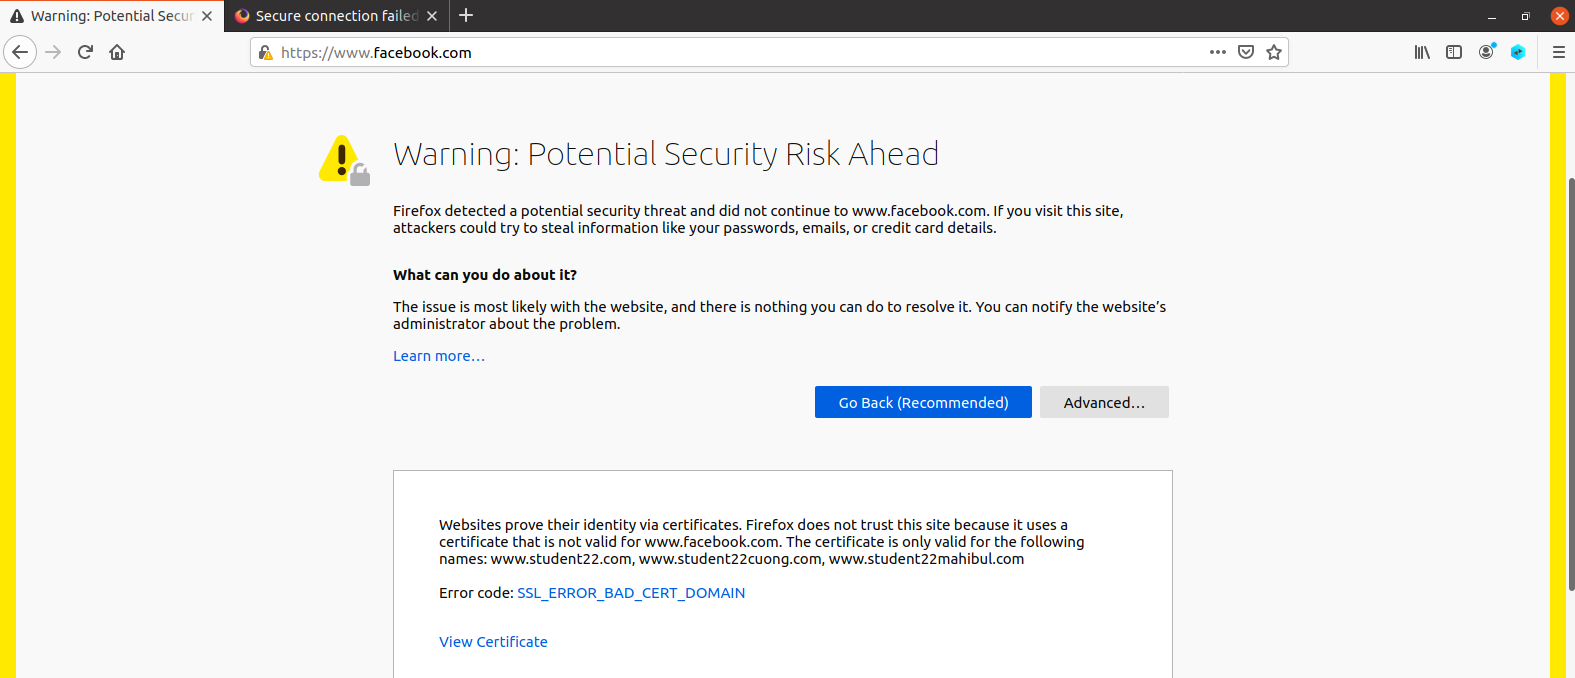
\includegraphics[height=\textheight,width=\textwidth,keepaspectratio]
    {figures/facebook_invalid_cert.png}
    \caption{Some issues while using the certificate binding to
    {\fontfamily{qcr}\selectfont www.facebook.com}}
    \label{fig:facebook_invalid}
\end{figure}

\begin{lstlisting}[caption=Append {\fontfamily{qcr}\selectfont
    www.facebook.com} to the list of known hosts,
    label={lst:facebook_dns}]
    10.9.0.80 www.facebook.com
\end{lstlisting}

In this work, we used {\fontfamily{qcr}\selectfont www.facebook.com} as the target
website. We appended the DNS name to the list of known hosts (see \autoref{lst:facebook_dns}).
As the certificate that we made in Task 3 did not include {\fontfamily{qcr}\selectfont
www.facebook.com} as one of valid DNS names, Firefox raised an error indicating the server
name is not included in the certificate issuing it (see \autoref{fig:facebook_invalid}).
Hence, the MITM attack did not work in this case.  